\documentclass[10pt]{article}
\usepackage[a4paper,margin=1.8cm]{geometry}
\usepackage{amsmath,amssymb,amsthm,mathtools,xcolor,tikz}
\usetikzlibrary{arrows.meta,positioning,calc}
\setlength{\parindent}{0pt}
\setlength{\parskip}{5pt}
\allowdisplaybreaks
\newcommand{\E}{\mathbb{E}}
\newcommand{\Pp}{\mathbb{P}}
\newcommand{\F}{\mathcal{F}}
\newcommand{\Hh}{\mathcal{H}}
\newcommand{\KL}{D_{\mathrm{KL}}}
\newcommand{\grad}{\nabla}
\newcommand{\on}{\theta_n}
\newcommand{\xs}{x^{(b)}}
\newcommand{\ys}{y^{(b,i)}}
\newcommand{\Ab}{\widehat A^{(b,i)}}
\newcommand{\rh}{\widehat\rho^{(b,i)}}
\newcommand{\rb}{\rho^{(b,i)}}
\newcommand{\un}{U_{n,b}}
\newcommand{\bn}{b_n}
\newtheoremstyle{preserved}{5pt}{5pt}{\normalfont}{} {\bfseries}{.}{0.5em}{}
\theoremstyle{preserved}
\newtheorem{assumption}{Assumption}
\newtheorem{lemma}{Lemma}
\newtheorem{proposition}{Proposition}
\newtheorem{theorem}{Theorem}
\newtheorem*{corollary}{Corollary: total bias bound}
\renewcommand{\qedsymbol}{}

\begin{document}
\section*{GMC-GRPO without Assumption 3}

Objective:
\begin{equation*}
J(\theta)=\E_{x\sim D}\E_{y\sim\pi_\theta(\cdot\mid x)}[r_\phi(x,y)].
\end{equation*}
\subsection*{Notation}
\begin{itemize}
\item $\theta\in\mathbb{R}^d$ policy parameters
\item $D$ training prompt distribution
\item $\pi_\theta(y\mid x)$ probability of generating $y$ given prompt $x$
\item $r_\phi(x,y)\in[0,R]$ reward assigned to that trajectory
\item $B$ number of returned groups / update
\item $G$ number of responses / group
\item $\tau_n^{(b)}$ delay of group $b$
\item $\F_n^-:=\sigma\bigl(\{\text{all info available before mini-batch used at iteration }n\text{ returned}\}\bigr)$
\item $\Hh_n:=\sigma\bigl(\F_n^-,\{x^{(b)},\tau_n^{(b)}\}_{b=1}^B\bigr).$
\end{itemize}

\subsection*{Proof notation lookup}

\begin{itemize}
    \item As in GMC--GRPO, we define $g_n$ as the gradient estimator:
\begin{equation*}
g_n:=\frac{1}{TBG}\sum_{b=1}^B\sum_{i=1}^G\rh\,\grad_\theta\log\pi_{\theta_n}(\ys\mid\xs)\,\Ab
\end{equation*}
where GMC importance ratio is
\begin{equation*}
\rh=\frac{\rb}{\max\bigl\{\frac{1}{1+\epsilon},\bar\rho_n^{(b)}\bigr\}},\qquad
\bar\rho_n^{(b)}=\frac1G\sum_{j=1}^G\rho^{(b,j)},\qquad
\rb=\frac{\pi_{\theta_n}(\ys\mid\xs)}{\pi_{\theta_{n-\tau_n^{(b)}}}(\ys\mid\xs)}.
\end{equation*}
\item LOO advantage:
\begin{equation*}
\Ab=r_\phi(\xs,\ys)-\frac1{G-1}\sum_{j\ne i}r_\phi(x^{(b)},y^{(b,j)}).
\end{equation*}
\item Group-level gradient estimators:
\begin{itemize}
    \item Group-level GMC estimator:
    \begin{equation*} U_{n,b}=\frac1{TG}\sum_{i=1}^G\rh\,\grad_\theta\log\pi_{\theta_n}(\ys\mid\xs)\Ab.
    \end{equation*}
    \item Raw importance sampling estimator:
    \begin{equation*}  U_{n,b}^{\mathrm{IS}}=\frac1{TG}\sum_{i=1}^G\rb\,\grad\log\pi_{\theta_n}(\ys\mid\xs)\Ab
    \end{equation*}
    \item Self-normalized estimator:
    \begin{equation*} U_{n,b}^{\mathrm{SN}}=\frac1{TG}\sum_{i=1}^G\frac{\rb}{\bar\rho_n^{(b)}}\grad\log\pi_{\theta_n}(\ys\mid\xs)\Ab.
    \end{equation*}
\end{itemize}
\item Bias terms:
\begin{itemize}
    \item Pathwise GMC correction bias: \begin{equation*} b_{n,b}^{\mathrm{corr}}:=U_{n,b}-U^{\mathrm{IS}}_{n,b}=\frac1{TG}\sum_{i=1}^G(\rh-\rb)\grad_\theta\log\pi_{\theta_n}(\ys\mid\xs)\Ab,
    \end{equation*}
    \item GMC correction bias: $$c_{n,b}:=\E[b_{n,b}^{\mathrm{corr}}\mid\Hh_n]=\E[U_{n,b}-U^{\mathrm{IS}}_{n,b}\mid\Hh_n]$$
    \item Sampling bias: \begin{equation*}
    s_{n,b}:=\E_{Q_{n,b}}[U_{n,b}^{\mathrm{IS}}\mid\Hh_n]-\frac1T\grad J_{x^{(b)}}(\theta_n)
    =\E_{Q_{n,b}}[U_{n,b}^{\mathrm{IS}}\mid\Hh_n]-\frac1T\E_{y\sim\pi_{\theta_n}(\cdot\mid\xs)}[r_\phi(\xs,y)\nabla \log \pi_{\theta_n}\left(y \mid x^{(b)}\right)].
    \end{equation*}
    \begin{itemize}
        \item[$\blacksquare$] We have \begin{equation*} \E[U_{n,b}\mid\Hh_n]=\frac1T\grad J_{x^{(b)}}(\theta_n)+s_{n,b}+c_{n,b}.\label{eq:step-2}
        \end{equation*}
    \end{itemize}
    \item Prompt-selection bias:
    \begin{equation*} p_n=\frac{1}{T} \mathbb{E}\left[\left.\frac{1}{B} \sum_{b=1}^B \nabla J_{x^{(b)}}\left(\theta_n\right) \right\rvert\, \mathcal{F}_n^{-}\right]-\frac{1}{T} \nabla J\left(\theta_n\right) 
    \end{equation*}
    \item Total bias: 
        \begin{align*}
        b_n &= \E[g_n\mid\F_n^-] - \frac{1}{T} \nabla J\left(\theta_n\right)\\&=\mathbb{E}\left[\left.\frac{1}{B} \sum_{b=1}^B \mathbb{E}\left[U_{n, b} \mid \mathcal{H}_n\right] \right\rvert\, \mathcal{F}_n^{-}\right]-\frac{1}{T} \nabla J\left(\theta_n\right) \\
        & =\mathbb{E}\left[\left.\frac{1}{B} \sum_{b=1}^B\left(\frac{1}{T} \nabla J_{x^{(b)}}\left(\theta_n\right)+s_{n, b}+c_{n, b}\right) \right\rvert\, \mathcal{F}_n^{-}\right]-\frac{1}{T} \nabla J\left(\theta_n\right) \\
        & =\frac{1}{T} \mathbb{E}\left[\left.\frac{1}{B} \sum_{b=1}^B \nabla J_{x^{(b)}}\left(\theta_n\right) \right\rvert\, \mathcal{F}_n^{-}\right]-\frac{1}{T} \nabla J\left(\theta_n\right) +\mathbb{E}\left[\left.\frac{1}{B} \sum_{b=1}^B\left(s_{n, b}+c_{n, b}\right) \right\rvert\, \mathcal{F}_n^{-}\right] \\
        &= p_n+\mathbb{E}\left[\left.\frac{1}{B} \sum_{b=1}^B\left(s_{n, b}+c_{n, b}\right) \right\rvert\, \mathcal{F}_n^{-}\right]
        \end{align*}
        \begin{itemize}
        \item[$\blacksquare$] We have \begin{align*}
        \E[g_n\mid\F_n^-]&=\frac1T\grad J(\theta_n)+b_n \\
        &=\frac1T\grad J(\theta_n)+\underbrace{p_n}_{\text{prompt selection bias}}+
    \E\left[\left.\frac1B\sum_{b=1}^B\left(\underbrace{s_{n,b}}_{\text{response selection bias}}+\underbrace{c_{n,b}}_{\text{GMC correction bias}}\right)\right|\F_n^-\right].
        \end{align*}
        \end{itemize} 
\end{itemize}
    \item Distributions:
    \begin{itemize}
        \item Reference distribution of the $G$ responses in group $b$: \begin{equation*}
        P_{n,b}=\pi_{\theta_{n-\tau_n^{(b)}}}(\cdot\mid x^{(b)})^{\otimes G}
        \end{equation*}
        This means that conditional on $x^{(b)}$ \& $\theta_{n-\tau_n^{(b)}}$,
        \begin{equation*} y^{(b,1)},\ldots,y^{(b,G)}\overset{\mathrm{iid}}\sim\pi_{\theta_{n-\tau_n^{(b)}}}(\cdot\mid x^{(b)}).
        \end{equation*}
        \item Define conditional joint dist. of group $b$:
        \begin{equation*} Q_{n,b}:=\mathcal{L}\left((y^{(b,1)},\ldots,y^{(b,G)})\mid\Hh_n\right)
        \end{equation*}
        \begin{equation*}
        \Rightarrow\quad Q_{n,b}(y^1,\ldots,y^G)\ne\prod_{i=1}^G\underbrace{Q^i_{n,b}(y^i)}_{=\Pp(y^{(b,i)}=y^i\mid\Hh_n)}
        \end{equation*}
        in general (if the observed delay reveals information about the group's maximum completion time, conditioning on it can couple the responses. For example, knowing the group took long may imply at least one response was long). Thus \underline{we do not assume} $y^{(b,i)}\mid\Hh_n\overset{\mathrm{iid}}\sim\pi_{\theta_{n-\tau_n^{(b)}}}(\cdot\mid\xs)$. Note that $Q_{n, b} \neq P_{n, b}$ can occur even if $Q_{n, b}$ factorizes (for example, a delay that indicates all responses finished within a fixed time window can change each response's marginal distribution without introducing dependence).
        \item $\Delta_{n,b}:=\chi^2(Q_{n,b}\|P_{n,b})$ assuming $Q_{n,b}\ll P_{n,b}$ and that the divergence is finite.
    \end{itemize}
\end{itemize}

\subsection*{Assumptions}

\begin{assumption}[Token-level Lipschitz score] $\exists L>0$ s.t. $\forall(x,y_{<t}),y_t$ and $\theta,\theta'\in\mathbb{R}^d$,
\begin{equation*}
\left\|\grad_\theta\log\pi_\theta(y_t\mid x,y_{<t})-\grad_\theta\log\pi_{\theta'}(y_t\mid x,y_{<t})\right\|_2\le L\|\theta-\theta'\|_2.
\end{equation*}
\end{assumption}
\begin{assumption}[Token-level coverage] $\exists C\ge1$ such that $\forall$ token, context, learner or behaviour policy used during training,
\begin{equation*}
\pi_\theta(y_t\mid x,y_{<t})\ge\frac1C.
\end{equation*}

\end{assumption}

\subsection*{Results and proofs}

\begin{lemma} Let $\theta_{n+1}=\theta_n+\eta g_n$ and define the conditional bias
\begin{equation*}
b_n:=\E[g_n\mid\F_n^-]-\frac1T\grad J(\theta_n).
\end{equation*}
Under Assumptions 1--2, we have 
\begin{equation*}
\frac1N\sum_{n=0}^{N-1}\E\bigl[\|\grad J(\theta_n)\|_2^2\bigr]
\le\frac{2T(J^*-\E[J(\theta_0)])}{\eta N}
+\frac{T^2}{N}\sum_{n=0}^{N-1}\Bigl(\eta RL(2\log|\mathcal A|+1)\E[\|g_n\|_2^2]+\E[\|b_n\|_2^2]\Bigr).
\end{equation*}
\textcolor{red}{(Remark: Actually not sure Assumption 2 is used - I don't see a need for it)}
\end{lemma}
\begin{proof}[Proof sketch]

By Lemma 4, Assumption 1 implies $\grad J$ is $L_J$-Lipschitz for $L_J:=TRL(2\log|\mathcal A|+1)$ and it follows that
\begin{equation*}
J(\theta_{n+1})\ge J(\theta_n)+\eta\langle\grad J(\theta_n),g_n\rangle-\frac{L_J\eta^2}{2}\|g_n\|_2^2.
\end{equation*}
Taking conditional expectations and substituting $\E[g_n\mid\F_n^-]=\frac1T\grad J(\theta_n)+b_n$ we obtain
\begin{equation*}
\E[J(\theta_{n+1})\mid\F_n^-]-J(\theta_n)
\ge\frac\eta T\|\grad J(\theta_n)\|_2^2+\eta\langle\grad J(\theta_n),b_n\rangle
-\frac{L_J\eta^2}{2}\E[\|g_n\|_2^2\mid\F_n^-].
\end{equation*}
Now by Young's inequality,
\begin{equation*}
\langle\grad J(\theta_n),b_n\rangle\ge-\frac1{2T}\|\grad J(\theta_n)\|_2^2-\frac T2\|b_n\|_2^2.
\end{equation*}
giving
\begin{equation*}
\E[J(\theta_{n+1})\mid\F_n^-]-J(\theta_n)
\ge\frac\eta{2T}\|\grad J(\theta_n)\|_2^2-\frac{\eta T}{2}\|b_n\|_2^2
-\frac{L_J\eta^2}{2}\E[\|g_n\|_2^2\mid\F_n^-].
\end{equation*}
Taking total expectations \& rearranging gives
\begin{equation*}
\frac\eta{2T}\E[\|\grad J(\theta_n)\|_2^2]
\le\E[J(\theta_{n+1})-J(\theta_n)]+\frac{\eta T}{2}\E[\|b_n\|_2^2]+\frac{L_J\eta^2}{2}\E[\|g_n\|_2^2].
\end{equation*}
Summing over $n=0,\ldots,N-1$ gives
\begin{equation*}
\frac\eta{2T}\sum_{n=0}^{N-1}\E[\|\grad J(\theta_n)\|_2^2]
\le\E[J(\theta_N)]-\E[J(\theta_0)]
+\sum_{n=0}^{N-1}\left(\frac{\eta T}{2}\E[\|b_n\|_2^2]+\frac{L_J\eta^2}{2}\E[\|g_n\|_2^2]\right).
\end{equation*}
Multiplying both sides by $\frac{2T}{\eta N}$ and using $J(\theta_N)\le J^*$ gives
\begin{equation*}
\frac1N\sum_{n=0}^{N-1}\E[\|\grad J(\theta_n)\|_2^2]
\le\frac{2T(J^*-\E[J(\theta_0)])}{\eta N}
+\frac{T^2}{N}\sum_{n=0}^{N-1}\Bigl(\E[\|b_n\|_2^2]+\eta RL(2\log|\mathcal A|+1)\E[\|g_n\|_2^2]\Bigr).\quad\square
\end{equation*}

\end{proof}

Define the weighted gradient estimator
\begin{equation*}
g_n=\frac1B\sum_{b=1}^B U_{n,b}
\end{equation*}
where
\begin{equation*}
U_{n,b}=\frac1{TG}\sum_{i=1}^G\rh\,\grad_\theta\log\pi_{\theta_n}(\ys\mid\xs)\Ab.
\end{equation*}
Note that $0\le\rh\le\rb$, $\frac1G\sum_{i=1}^G\rh\le1+\epsilon$.

\begin{proposition}[Adapted] Under Assumptions 1--2, the GMC estimator satisfies
\begin{equation*} \|g_n\|_2^2 \le8R^2(1+\epsilon)^2L\log C \quad
\end{equation*}
almost surely.
Furthermore, defining
\begin{equation*}
b_{n,b}^{\mathrm{corr}}:=\frac1{TG}\sum_{i=1}^G(\rh-\rb)\grad_\theta\log\pi_{\theta_n}(\ys\mid\xs)\Ab,
\end{equation*}
we have
\begin{equation*}
\|\E[b_{n,b}^{\mathrm{corr}}\mid\Hh_n]\|_2
\le2R\sqrt{2L\log C}\,\E\left[\left.\frac1G\sum_{i=1}^G(\rb-\rh)\right|\Hh_n\right].
\end{equation*}
Both inequalities hold for arbitrary conditional expectations $Q_{n,b}$.
\end{proposition}
\textcolor{red}{(Remark: Also substitutes for Lemma 5, which is a GMC-specific version of Proposition 1)}

\textcolor{blue}{Strategy: The original proof changes measure from the behaviour policy to the current policy using Assumption 3.
I replaced this with a pathwise bound using Lemma 2 and the GMC mass cap from Assumptions 1-2:
$$
\left\|g_n\right\|^2 \leq 8 R^2(1+\epsilon)^2 L \log C .
$$
This holds regardless of the returned-group distribution.}

\begin{proof} \underline{Step 1 (exactly same as paper)} Applying weighted Cauchy--Schwarz to $U_{n,b}$,
\begin{equation*}
\|U_{n,b}\|_2^2\le\left(\frac1G\sum_{i=1}^G\rh\right)
\left(\frac1G\sum_{i=1}^G\rh\left\|\frac1T\grad\log\pi_{\theta_n}(\ys\mid\xs)\Ab\right\|_2^2\right).
\end{equation*}
\underline{Step 2 (where our proof differs)} The paper uses $\hat\rho\le\rho$ and changes measure from behaviour policy to current policy.

This requires Assumption 3. Instead, use $\|\grad_\theta\log\pi_\theta(y\mid x)\|_2\le T\sqrt{2L\log C}$ from Lemma 2 and $|\Ab|\le2R$:
\begin{equation*}
\left\|\frac1T\grad\log\pi_{\theta_n}(\ys\mid\xs)\Ab\right\|_2^2
\le2L\log C\cdot4R^2=8R^2L\log C.
\end{equation*}
\begin{equation}\label{eq:score-bound}
\begin{aligned}
\Rightarrow\quad\|U_{n,b}\|_2^2
&\le\left(\frac1G\sum_{i=1}^G\rh\right)^2(8R^2L\log C)\\
&\le(1+\epsilon)^2(8R^2L\log C).\qquad
\end{aligned}
\end{equation}
\underline{Step 3 (exactly same as paper)} By Convexity,
\begin{equation*}
\|g_n\|_2^2\le\frac1B\sum_{b=1}^B\|U_{n,b}\|_2^2\le8R^2(1+\epsilon)^2L\log C.
\end{equation*}
\underline{Step 4 (exactly same as paper)} For correction term, since $\rb-\rh\ge0$, conditional Jensen + uniform score bound (Lemma 2) give
\begin{equation*}
\begin{aligned}
\|\E[b_{n,b}^{\mathrm{corr}}\mid\Hh_n]\|_2
&\le\E[\|b_{n,b}^{\mathrm{corr}}\|_2\mid\Hh_n]\\
&\le2R\sqrt{2L\log C}\,\E\left[\left.\frac1G\sum_{i=1}^G(\rb-\rh)\right|\Hh_n\right].\quad\square
\end{aligned}
\end{equation*}

\end{proof}

\textcolor{blue}{Strategy: originally, importance sampling is conditionally unbiased, so only the GMC correction causes bias. Since Assumption 3 doesn't hold, total bias now decomposes into three components: the prompt-selection bias $p_n$, response-selection bias $s_{n,b}$ and GMC correction bias $c_{n,b}$.}

\setcounter{proposition}{2}
\begin{proposition}[Adapted] Define raw importance sampling estimator
\begin{equation*}
U_{n,b}^{\mathrm{IS}}=\frac1{TG}\sum_{i=1}^G\rb\,\grad\log\pi_{\theta_n}(\ys\mid\xs)\Ab
\end{equation*}
and self-normalized estimator
\begin{equation*}
U_{n,b}^{\mathrm{SN}}=\frac1{TG}\sum_{i=1}^G\frac{\rb}{\bar\rho_n^{(b)}}\grad\log\pi_{\theta_n}(\ys\mid\xs)\Ab.
\end{equation*}
Under Assumption 1 (without Assumption 3) the following pointwise identity holds:
\begin{equation}
 U_{n,b}-U_{n,b}^{\mathrm{IS}}=-\left(\bar\rho_n^{(b)}-(1+\epsilon)\right)_+U_{n,b}^{\mathrm{SN}}.\label{eq:step-1}
\end{equation}
Define the sampling bias
\begin{equation*}
s_{n,b}:=\E_{Q_{n,b}}[U_{n,b}^{\mathrm{IS}}\mid\Hh_n]-\frac1T\grad J_{x^{(b)}}(\theta_n)
=\E_{Q_{n,b}}[U_{n,b}^{\mathrm{IS}}\mid\Hh_n]-\frac1T\E_{y\sim\pi_{\theta_n}(\cdot\mid\xs)}[r_\phi(\xs,y)\nabla \log \pi_{\theta_n}\left(y \mid x^{(b)}\right)].
\end{equation*}
Recall from Proposition 1
\begin{equation*}
b_{n,b}^{\mathrm{corr}}=\frac1{TG}\sum_{i=1}^G(\rh-\rb)\grad\log\pi_{\theta_n}(\ys\mid\xs)\Ab=U_{n,b}-U^{\mathrm{IS}}_{n,b}.
\end{equation*}
Define $c_{n,b}:=\E[b_{n,b}^{\mathrm{corr}}\mid\Hh_n]$.

Then
\begin{equation}
\E[U_{n,b}\mid\Hh_n]=\frac1T\grad J_{x^{(b)}}(\theta_n)+s_{n,b}+c_{n,b}.\label{eq:step-2}
\end{equation}
Furthermore, define the prompt-selection bias
\begin{equation}
p_n:=\frac1T\left(\E\left[\left.\frac1B\sum_{b=1}^B\grad J_{x^{(b)}}(\theta_n)\right|\F_n^-\right]-\grad J(\theta_n)\right).\label{eq:step-3}
\end{equation}
Then $\E[g_n\mid\F_n^-]=\frac1T\grad J(\theta_n)+b_n$
\begin{equation}
=\frac1T\grad J(\theta_n)+\underbrace{p_n}_{\text{prompt selection bias}}+
\E\left[\left.\frac1B\sum_{b=1}^B\left(\underbrace{s_{n,b}}_{\text{response selection bias}}+\underbrace{c_{n,b}}_{\text{GMC correction bias}}\right)\right|\F_n^-\right].\label{eq:step-4}
\end{equation}

\end{proposition}

\begin{proof} \underline{Step 1}\quad Proving \eqref{eq:step-1} is exactly same as paper (see page 28).

\underline{Step 2}\quad Proving \eqref{eq:step-2}: From definition of $b_{n,b}^{\mathrm{corr}}$ we have
\begin{equation*}
U_{n,b}=U_{n,b}^{\mathrm{IS}}+\underbrace{b_{n,b}^{\mathrm{corr}}}_{=c_{n,b}\text{ in expectation}}
\end{equation*}
\begin{equation*}
\begin{aligned}
\Rightarrow\quad\E[U_{n,b}\mid\Hh_n]&=\E[U_{n,b}^{\mathrm{IS}}\mid\Hh_n]+\underbrace{\E[b_{n,b}^{\mathrm{corr}}\mid\Hh_n]}_{=c_{n,b}}\\
&=\frac1T\grad J_{x^{(b)}}(\theta_n)+s_{n,b}+c_{n,b}.
\end{aligned}
\end{equation*}
\underline{Step 3}\quad Proving \eqref{eq:step-4}: Since $\F_n^-\subseteq\Hh_n$, by tower property
\begin{equation*}
\begin{aligned}
\E[g_n\mid\F_n^-]
&=\frac1B\E\left[\left.\sum_{b=1}^B U_{n,b}\right|\F_n^-\right]\\
&=\frac{1}{TB}\E\left[\left.\sum_{b=1}^B\grad J_{x^{(b)}}(\theta_n)\right|\F_n^-\right]
+\frac1B\E\left[\left.\sum_{b=1}^B(s_{n,b}+c_{n,b})\right|\F_n^-\right]
\end{aligned}
\end{equation*}
Substituting \eqref{eq:step-3}, we get
\begin{equation*}
\E[g_n\mid\F_n^-]=\frac1T\grad J(\theta_n)+p_n+\frac1B\E\left[\left.\sum_{b=1}^B(s_{n,b}+c_{n,b})\right|\F_n^-\right].\quad\square
\end{equation*}

\end{proof}

Define a reference distribution conditional on $\Hh_n$:
\begin{equation*}
P_{n,b}=\pi_{\theta_{n-\tau_n^{(b)}}}(\cdot\mid x^{(b)})^{\otimes G}
\end{equation*}
and recall
\begin{equation*}
Q_{n,b}=\mathcal L\bigl((y^{(b,1)},\ldots,y^{(b,G)})\mid\Hh_n\bigr).
\end{equation*}

\setcounter{lemma}{5}
\begin{lemma}[Adapted] Define $\Delta_{n,b}:=\chi^2(Q_{n,b}\|P_{n,b})$ assuming $Q_{n,b}\ll P_{n,b}$ and that the divergence is finite.

Under Assumptions 1--2, the total group-level conditional bias from Proposition 3 satisfies
\begin{equation*}
\|s_{n,b}+c_{n,b}\|_2^2\le
\frac{16R^2L\log C}{\log^2(1+2\epsilon)}(D_n^{(b)})^2
+16R^2(1+\epsilon)^2L\log C\,\Delta_{n,b}
\end{equation*}
where $D_n^{(b)}:=\KL\bigl(\pi_{\theta_n}\|\pi_{\theta_{n-\tau_n^{(b)}}}\bigr)$.

\end{lemma}

\textcolor{blue}{Strategy: Apply the result of original Lemma 6 under a hypothetical reference distribution $P_{n, b}$, then bound the difference from the actual distribution $Q_{n, b}$ using Cauchy-Schwarz:
$$
\left\|s_{n, b}+c_{n, b}\right\|^2 \leq \underbrace{C_1\left(D_n^{(b)}\right)^2}_{\text {original KL contribution }}+\underbrace{C_2 \Delta_{n, b}}_{\text {new response-selection term }},
$$
where $\Delta_{n, b}=\chi^2\left(Q_{n, b} \| P_{n, b}\right)$.}

\begin{proof} From Proposition 3,
\begin{equation}\label{eq:bias-decomposition}
\begin{aligned}
s_{n,b}+c_{n,b}&=\E_{Q_{n,b}}[U_{n,b}\mid\Hh_n]-\frac1T\grad J_{x^{(b)}}(\theta_n)\\
&=\underbrace{\left(\E_{P_{n,b}}[U_{n,b}\mid\Hh_n]-\frac1T\grad J_{x^{(b)}}(\theta_n)\right)}_{=(I)}
+\underbrace{\left(\E_{Q_{n,b}}[U_{n,b}\mid\Hh_n]-\E_{P_{n,b}}[U_{n,b}\mid\Hh_n]\right)}_{=(II)}.
\end{aligned}
\end{equation}
Now (I) is the reference GMC correction bias, $b_{n,b}^{\mathrm{P_{n,b}}}:=\E_{P_{n,b}}[b_{n,b}^{\mathrm{corr}}\mid\Hh_n]$:
\begin{align*}(I) & =\E_{P_{n,b}}\left[U_{n, b} \mid \mathcal{H}_n\right]-\frac{1}{T} \nabla J_{x^{(b)}}\left(\theta_n\right) \\ & =\E_{P_{n,b}}\left[U_{n, b}-U_{n, b}^{\mathrm{IS}} \mid \mathcal{H}_n\right] \\ & =b_{n, b}^P,\end{align*}
so the paper's conditional i.i.d. argument holds and we can apply Lemma 6:
\begin{equation*}
\|(I)\|_2^2\le\frac{8R^2L\log C}{\log^2(1+2\epsilon)}(D_n^{(b)})^2.
\end{equation*}
\textcolor{red}{(Remark: Chose this branch of Lemma 6 to recover delay dependence as in original Theorem 1. Could keep all 4 for stronger result, but in the paper they also chose this branch for Theorem 1. Theorem 3 retains the full minimum.)}

Now to bound (II), let $R_{n,b}=dQ_{n,b}/dP_{n,b}$,
\begin{equation}
\begin{aligned}
(II)&=\E_{P_{n,b}}[R_{n,b}U_{n,b}\mid\Hh_n]-\E_{P_{n,b}}[U_{n,b}\mid\Hh_n]\\
&=\E_{P_{n,b}}[(R_{n,b}-1)U_{n,b}\mid\Hh_n].
\end{aligned}\label{eq:step-6}
\end{equation}
$\Rightarrow$ by Cauchy--Schwarz
\begin{equation}
\begin{aligned}
\|(II)\|_2^2
&\le\E_{P_{n,b}}[(R_{n,b}-1)^2\mid\Hh_n]\E_{P_{n,b}}[\|U_{n,b}\|_2^2\mid\Hh_n]\\
&=\E_{P_{n,b}}\left[\left.\left(\frac{dQ_{n,b}}{dP_{n,b}}-1\right)^2\right|\Hh_n\right]\E_{P_{n,b}}[\|U_{n,b}\|_2^2\mid\Hh_n]\\
&\le\Delta_{n,b}\cdot8R^2(1+\epsilon)^2L\log C,
\end{aligned}\label{eq:step-7}
\end{equation}
where we used \eqref{eq:score-bound} for 2nd term.

Finally using $\|a+b\|_2^2\le2\|a\|_2^2+2\|b\|_2^2$ in \eqref{eq:bias-decomposition} and substituting \eqref{eq:step-6} and \eqref{eq:step-7} we get
\begin{equation*}
\|s_{n,b}+c_{n,b}\|_2^2\le\frac{16R^2L\log C}{\log^2(1+2\epsilon)}(D_n^{(b)})^2+16R^2(1+\epsilon)^2L\log C\,\Delta_{n,b}.\quad\square
\end{equation*}
\end{proof}

\begin{corollary} Recall $b_n=p_n+\E[\frac1B\sum_{b=1}^B(s_{n,b}+c_{n,b})\mid\F_n^-]$
\begin{equation*}
\begin{aligned}
\Rightarrow\quad\|b_n\|_2^2
&\le2\|p_n\|_2^2+2\left\|\E\left[\left.\frac1B\sum_{b=1}^B(s_{n,b}+c_{n,b})\right|\F_n^-\right]\right\|_2^2\\
&\le2\|p_n\|_2^2+2\E\left[\left.\left\|\frac1B\sum_{b=1}^B(s_{n,b}+c_{n,b})\right\|_2^2\right|\F_n^-\right]\quad(\text{Jensen})\\
&\le2\|p_n\|_2^2+\frac2B\sum_{b=1}^B\E[\|s_{n,b}+c_{n,b}\|_2^2\mid\F_n^-]\quad(\text{convexity})\\
&\le2\|p_n\|_2^2+\frac2B\sum_{b=1}^B\E\left[\left.\frac{16R^2L\log C}{\log^2(1+2\epsilon)}(D_n^{(b)})^2+16R^2(1+\epsilon)^2L\log C\,\Delta_{n,b}\right|\F_n^-\right].\quad\square
\end{aligned}
\end{equation*}

\end{corollary}

\setcounter{lemma}{6}
\begin{lemma}[Adapted] Under Assumptions 1--2 and GMC update rule, without Assumption 3, we obtain
\begin{equation*}
D_n^{(b)}\le4(1+\epsilon)^2TR^2L^2\log C\,\eta^2(\tau_n^{(b)})^2.
\end{equation*}
Consequently,
\begin{equation*}
\E[(D_n^{(b)})^2\mid\tau_n^{(b)}]\le16(1+\epsilon)^4T^2R^4L^4(\log C)^2\eta^4(\tau_n^{(b)})^4.
\end{equation*}
\end{lemma}

\textcolor{blue}{Strategy: Original Lemma 7 uses an expected bound on the second moment of $g$ and uses Assumption 3 to separate the delay from the parameter updates. This obtains a tighter exponent $(1 + \epsilon)^3$. We instead use a pathwise bound $\|g_s\|^2\le 8R^2(1+\epsilon)^2L\log C$ and substitute this directly into 
$$
\|\theta_n-\theta_{n-\tau}\|^2
\le\eta^2\tau\sum_{s=n-\tau}^{n-1}\|g_s\|^2,
$$ 
which does not require independence between delays and previous updates.}

\begin{proof} Fix $t=\tau_n^{(b)}$. As in original proof,
\begin{equation*}
\theta_n-\theta_{n-t}=\eta\sum_{s=n-t}^{n-1}g_s.
\end{equation*}
Cauchy--Schwarz gives
\begin{equation*}
\|\theta_n-\theta_{n-t}\|_2^2\le\eta^2t\sum_{s=n-t}^{n-1}\|g_s\|_2^2.
\end{equation*}
Using the pathwise bound established in adapted Proposition 1,
\begin{equation}
\begin{aligned}
\|\theta_n-\theta_{n-t}\|_2^2
&\le\eta^2t\sum_{s=n-t}^{n-1}8R^2(1+\epsilon)^2L\log C\\
&=8R^2(1+\epsilon)^2L\log C\,\eta^2t^2.\label{eq:step-8}
\end{aligned}
\end{equation}
Now Lemma 3 with \eqref{eq:step-8} gives
\begin{equation*}
\begin{aligned}
D_n^{(b)}&\le\frac{TL}{2}\|\theta_n-\theta_{n-t}\|_2^2\\
&\le\frac{TL}{2}\,8R^2(1+\epsilon)^2L\log C\,\eta^2t^2
=4TR^2(1+\epsilon)^2L^2\log C\,\eta^2t^2.
\end{aligned}
\end{equation*}
Squaring gives the pointwise bound
\begin{equation*}
(D_n^{(b)})^2\le\left(4T R^2L^2(1+\epsilon)^2\log C\,\eta^2t^2\right)^2
\end{equation*}
so that
\begin{equation*}
\E[(D_n^{(b)})^2\mid\tau_n^{(b)}=t]\le16T^2L^4R^4(1+\epsilon)^4(\log C)^2\eta^4t^4.\quad\square
\end{equation*}
\end{proof}

Now let
\begin{equation*}
\overline{\tau^4}:=\frac1{NB}\sum_{n=0}^{N-1}\sum_{b=1}^B\E[(\tau_n^{(b)})^4],\qquad
\overline\Delta:=\frac1{NB}\sum_{n=0}^{N-1}\sum_{b=1}^B\E[\Delta_{n,b}],\qquad
\overline P:=\frac1N\sum_{n=0}^{N-1}\E[\|p_n\|_2^2].
\end{equation*}
\begin{theorem}[Adapted] Suppose Assumptions 1--2 hold and the learner uses GMC estimator $g_n$. Assume $\Delta_{n,b}<\infty$ $\forall 0\le n<N$, $1\le b\le B$.

Then, $\forall\eta>0$ and $N\ge1$,
\begin{equation*}
\frac1N\sum_{n=0}^{N-1}\E[\|\grad J(\theta_n)\|_2^2]
\le\frac{2T(J^*-\E[J(\theta_0)])}{\eta N}+C_1\eta+C_2\eta^4\overline{\tau^4}+C_3\overline\Delta+2T^2\overline P,
\quad\text{where}
\end{equation*}

\begin{equation*}
C_1=8T^2R^3L^2(1+\epsilon)^2\log C(2\log|\mathcal A|+1),
\end{equation*}
\begin{equation*}
C_2=\frac{512T^4R^6L^5(1+\epsilon)^4(\log C)^3}{\log^2(1+2\epsilon)}\qquad\text{and}
\end{equation*}
\begin{equation*}
C_3=32T^2R^2L(1+\epsilon)^2\log C.
\end{equation*}
\end{theorem}
\begin{proof} Recall Lemma 1 gives
\begin{equation*}
\frac1N\sum_{n=0}^{N-1}\E[\|\grad J(\theta_n)\|_2^2]
\le\frac{2T(J^*-\E[J(\theta_0)])}{\eta N}+
\frac{T^2}{N}\sum_{n=0}^{N-1}\left(\eta RL(2\log|\mathcal A|+1)\E[\|g_n\|_2^2]+\E[\|b_n\|_2^2]\right).
\end{equation*}
Now from Proposition 1,
\begin{equation*}
\E[\|g_n\|_2^2]\le8R^2(1+\epsilon)^2L\log C
\end{equation*}
\begin{equation}
\begin{aligned}
\Rightarrow\quad\frac{T^2}{N}\sum_n\eta RL(2\log|\mathcal A|+1)\E[\|g_n\|_2^2]
&\le8T^2\eta R^3L^2(2\log|\mathcal A|+1)(1+\epsilon)^2\log C\\
&=:C_1\eta.\label{eq:step-9}
\end{aligned}
\end{equation}
To bound the bias term, adapted Lemma 6 (Corollary) gave
\begin{equation*}
\|b_n\|_2^2\le2\|p_n\|_2^2+\frac2B\sum_{b=1}^B\E\left[\left.\frac{16R^2L\log C}{\log^2(1+2\epsilon)}(D_n^{(b)})^2+16R^2(1+\epsilon)^2L\log C\,\Delta_{n,b}\right|\F_n^-\right].
\end{equation*}
From adapted Lemma 7,
\begin{equation*}
(D_n^{(b)})^2\le16T^2L^4R^4(1+\epsilon)^4(\log C)^2\eta^4(\tau_n^{(b)})^4.
\end{equation*}
Substituting into the previous equation, taking expectations and multiplying by $T^2/N$ gives
\begingroup\small
\begin{equation}
\begin{aligned}
\frac{T^2}{N}\sum_n\E[\|b_n\|_2^2]
&\le\frac{2T^2}{N}\sum_n\E[\|p_n\|_2^2]
+\frac1{NB}\sum_{n=0}^{N-1}\sum_{b=1}^B\E\left[\frac{512T^4R^6L^5(1+\epsilon)^4(\log C)^3}{\log^2(1+2\epsilon)}\eta^4(\tau_n^{(b)})^4
+32T^2R^2(1+\epsilon)^2L\log C\,\Delta_{n,b}\right]\\
&=2T^2\overline P+\frac{512T^4R^6L^5(1+\epsilon)^4(\log C)^3}{\log^2(1+2\epsilon)}\eta^4\overline{\tau^4}
+32T^2R^2(1+\epsilon)^2L\log C\,\overline\Delta.\label{eq:step-10}
\end{aligned}
\end{equation}
\endgroup
Substituting \eqref{eq:step-9} and \eqref{eq:step-10} into Lemma 1 gives the result. $\square$

\end{proof}

\newpage

\subsection*{Proof dependency diagram}
\begin{center}
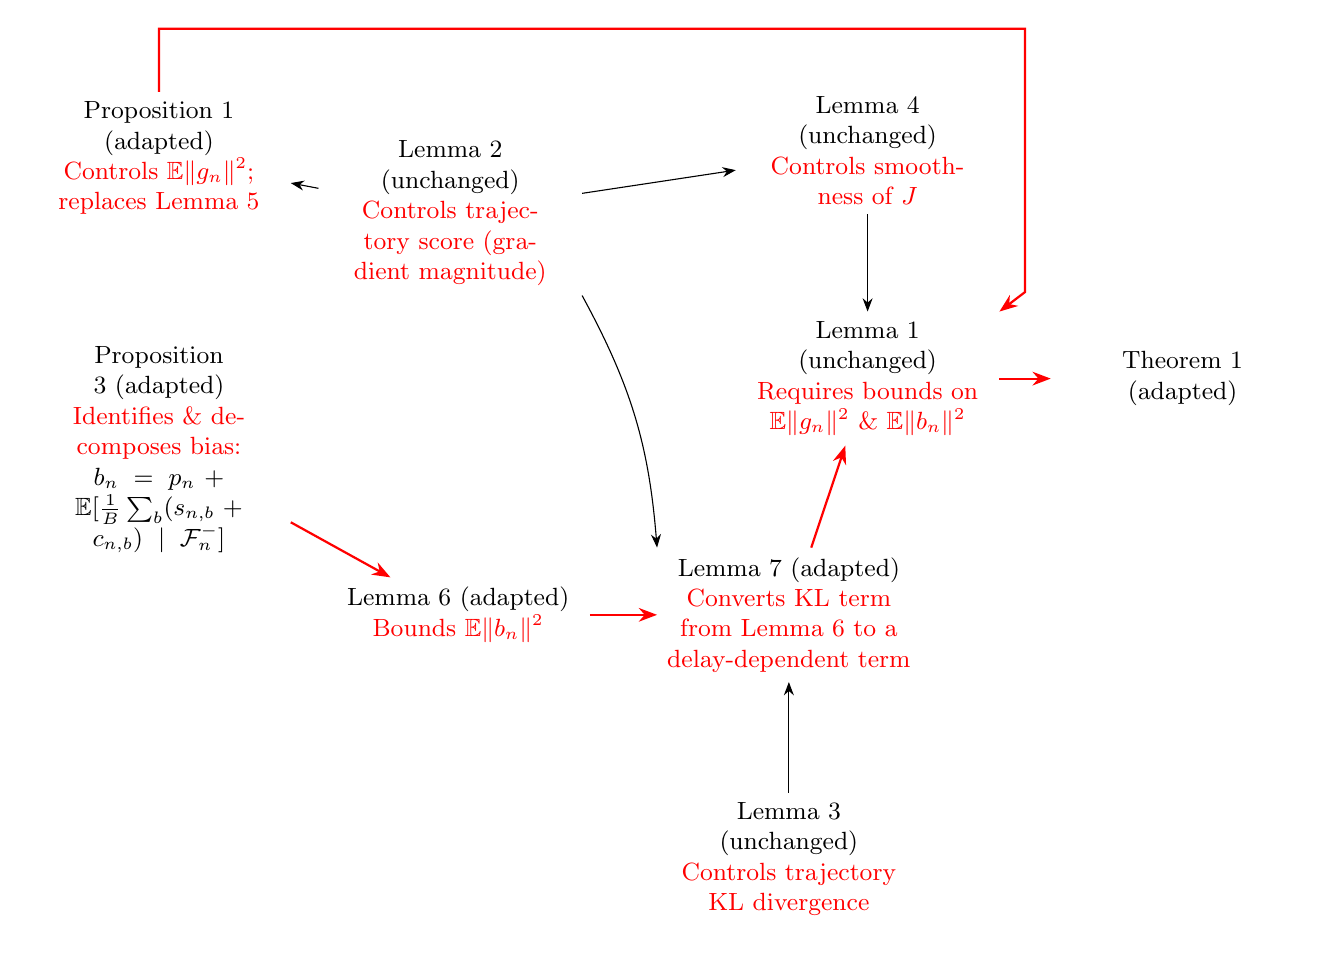
\begin{tikzpicture}[>=Stealth, node distance=2cm, every node/.style={align=center,font=\small},box/.style={text width=3.1cm}]
\node[box] (p1) at (0,4.5) {Proposition 1\\(adapted)\\\textcolor{red}{Controls $\E\|g_n\|^2$; replaces Lemma 5}};
\node[box] (l2) at (3.7,3.8) {Lemma 2 (unchanged)\\\textcolor{red}{Controls trajectory score (gradient magnitude)}};
\node[box] (l4) at (9,4.6) {Lemma 4 (unchanged)\\\textcolor{red}{Controls smoothness of $J$}};
\node[box] (p3) at (0,0.8) {Proposition 3 (adapted)\\\textcolor{red}{Identifies \& decomposes bias:}\\$b_n=p_n+\E[\frac1B\sum_b(s_{n,b}+c_{n,b})\mid\F_n^-]$};
\node[box] (l6) at (3.8,-1.3) {Lemma 6 (adapted)\\\textcolor{red}{Bounds $\E\|b_n\|^2$}};
\node[box] (l7) at (8,-1.3) {Lemma 7 (adapted)\\\textcolor{red}{Converts KL term from Lemma 6 to a delay-dependent term}};
\node[box] (l3) at (8,-4.4) {Lemma 3 (unchanged)\\\textcolor{red}{Controls trajectory KL divergence}};
\node[box] (l1) at (9,1.7) {Lemma 1 (unchanged)\\\textcolor{red}{Requires bounds on $\E\|g_n\|^2$ \& $\E\|b_n\|^2$}};
\node[box] (thm) at (13,1.7) {Theorem 1\\(adapted)};
\draw[->,red,thick] (p1.north) -- ++(0,0.8) -| (11,2.8) -- (l1.north east);
\draw[->] (l2) -- (p1);
\draw[->] (l2) -- (l4);
\draw[->] (l2.south east) to[bend left=12] (l7.north west);
\draw[->] (l4) -- (l1);
\draw[->,red,thick] (p3) -- (l6);
\draw[->,red,thick] (l6) -- (l7);
\draw[->,red,thick] (l7) -- (l1);
\draw[->] (l3) -- (l7);
\draw[->,red,thick] (l1) -- (thm);
\end{tikzpicture}
\end{center}
\end{document}